\documentclass{article}
\usepackage[utf8]{inputenc}
\usepackage{graphicx}

\title{Clases}
\author{Paubla Andrea Rivera Anaya }
\date{July 2020}

\begin{document}

\maketitle

\section{Nivel 1}

\begin{figure}[h!]
\centering
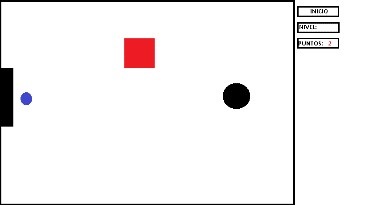
\includegraphics[width=1.1\textwidth]{1.jpg}
\caption{\label{fig1}Nivel 1}
\end{figure}
\\
Clases:
GraphicView, Manejo de escenas: en primera instancia 
Detección de colisiones.
\\
Clase 1: Obstáculo cuadrado 
\\
Clase 2: Objeto Tiro parabólico //comportamiento conjunto entre resorte y tiro parabólico.
\\
Clase 3: Obstáculo objetivo.
\\
Descripción: el desarrollo de este mundo se va llevar acabo aprendiendo el manejo de GraphicView, lo segundo es agregar las clases para los objetos dentro de este GraphicView. Antes de hacer este paso se harán las pruebas necesarias para ver el comportamiento de cada clase. Detectar colisiones entre clases.
\\
\section{Nivel 2}

\begin{figure}[h!]
\centering
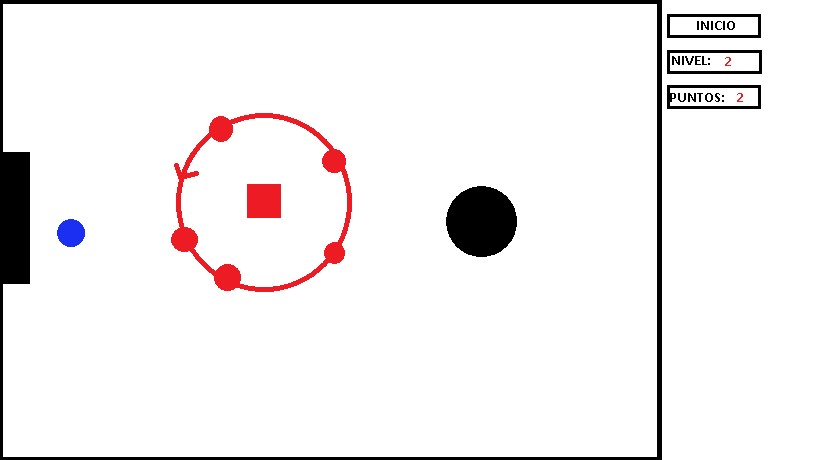
\includegraphics[width=1.1\textwidth]{2.jpg}
\caption{\label{fig1}Nivel 2}
\end{figure}
\\

Anexar:
Clase 4: Objeto con trayectoria circular.
Descripción: se debe tener en cuenta la colisión con este objeto también.

\section{Nivel 3}

\begin{figure}[h!]
\centering
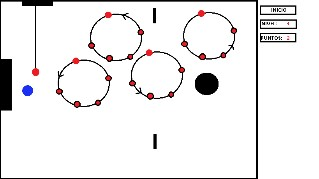
\includegraphics[width=1.1\textwidth]{3.jpg}
\caption{\label{fig1}Nivel 3}
\end{figure}
\\

Clase 5: Obstáculo péndulo.

\end{document}
